% !TEX root=../thesis.tex

\chapter{Background}


%Piloting map service for navigating in punctuality analysis for trains

A train network is a complex system. Almost every running train have the 
possibility to affect almost every other train running in the system.  When you look at a busy area, such as a major city and it's closest
area, a great deal of material can be on the move at any given time on a
rail network with limited capacity. This leads to limited time slots for each train and every
problem can lead to major problems, not just for the train experiencing the
problem, but can spread to other trains. \\

To minimize delays it may be necessary to improve both infrastructure and/or
time table on railway routes or parts of routes. However, to understand what
needs to be improved and optionally where, you need a good tool to analyze the
rail network capacity, and if necessary, visualize each individual train (see \vref{fig:zugmonitor}) in the rail network to follow delays to the source.

Here they have plotted each train on it's course between each station on it's
route, with a colored circle around the train which varies depending on if the
train is on schedule or delayed. It is also possible to play through the
selected day or drag through time manually.

\begin{figure}[!htbp]
	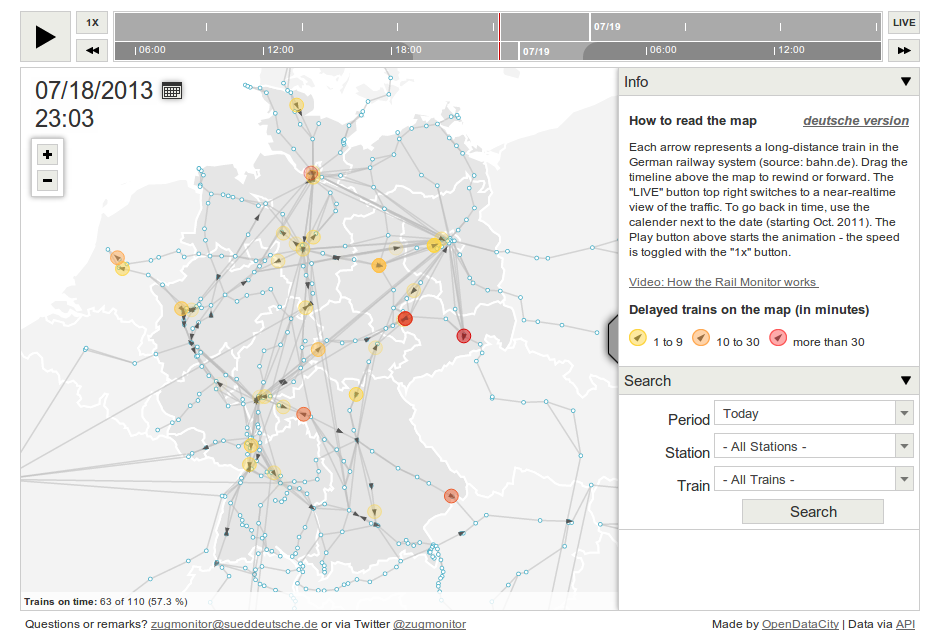
\includegraphics[width=\textwidth,center]{zugmonitor.png}
	\caption[Zugmonitor]{Zugmonitor \cite{zugmonitor}}
	\label{fig:zugmonitor}
\end{figure}

\begin{figure}[!htbp]
	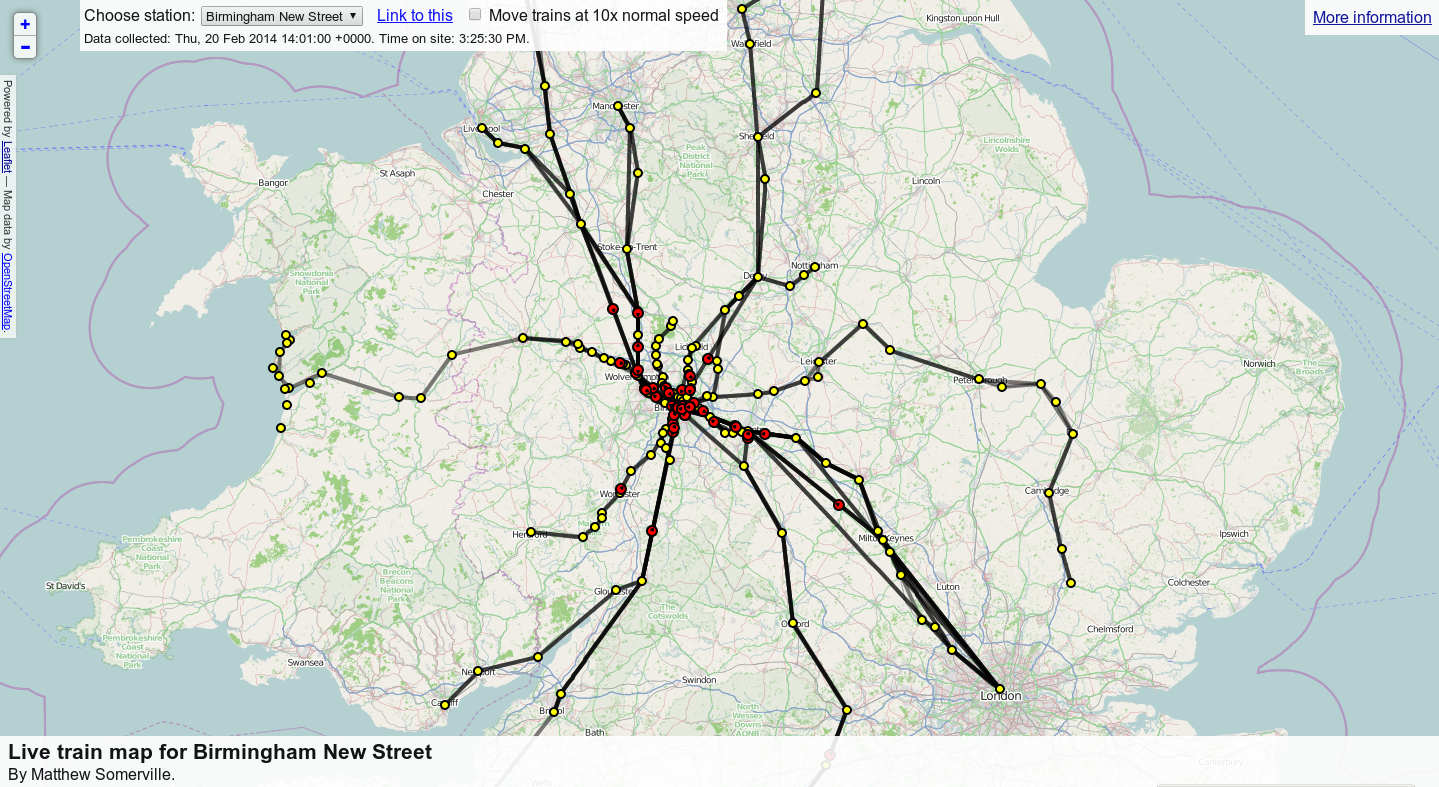
\includegraphics[width=\textwidth,center]{live-train-map-for-Birminingham-new-street.png}
	\caption[Live train map for Birmingham new street]{Live train map for Birmingham new street \cite{birminghamLiveMap}}
	\label{fig:birminghamLiveMap}
\end{figure}

\begin{figure}[!htbp]
	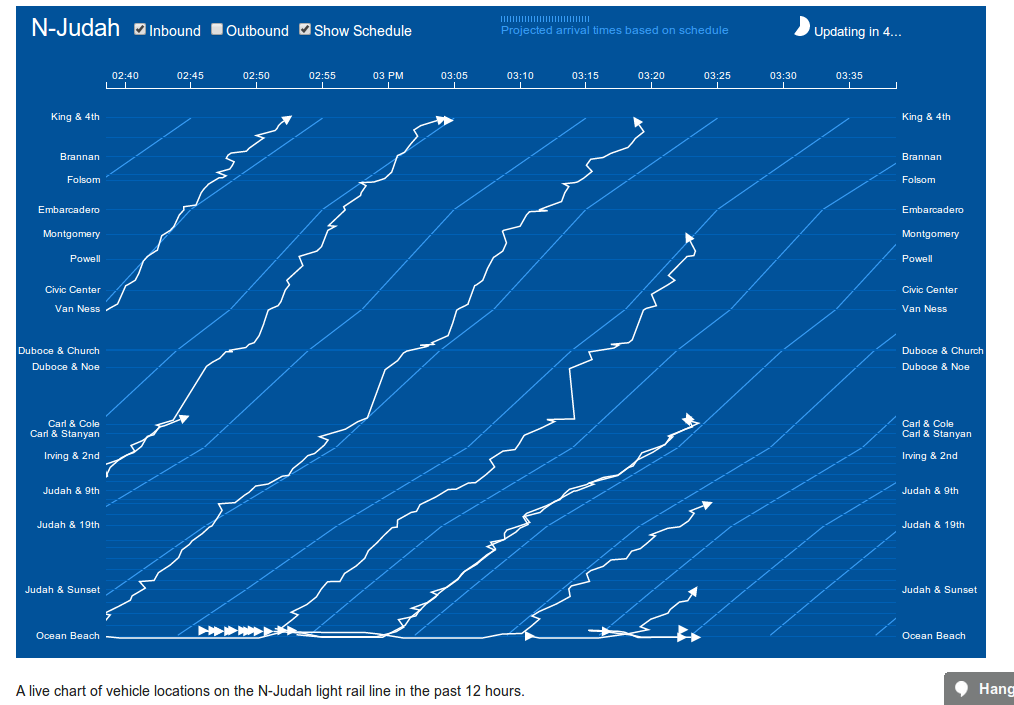
\includegraphics[width=\textwidth,center]{visualizing-transit-delays.png}
	\caption[Visualizing transit delays]{Visualizing transit delays \cite{muniLightRail}}
	\label{fig:muniLightRail}
\end{figure}

\begin{figure}[!htbp]
	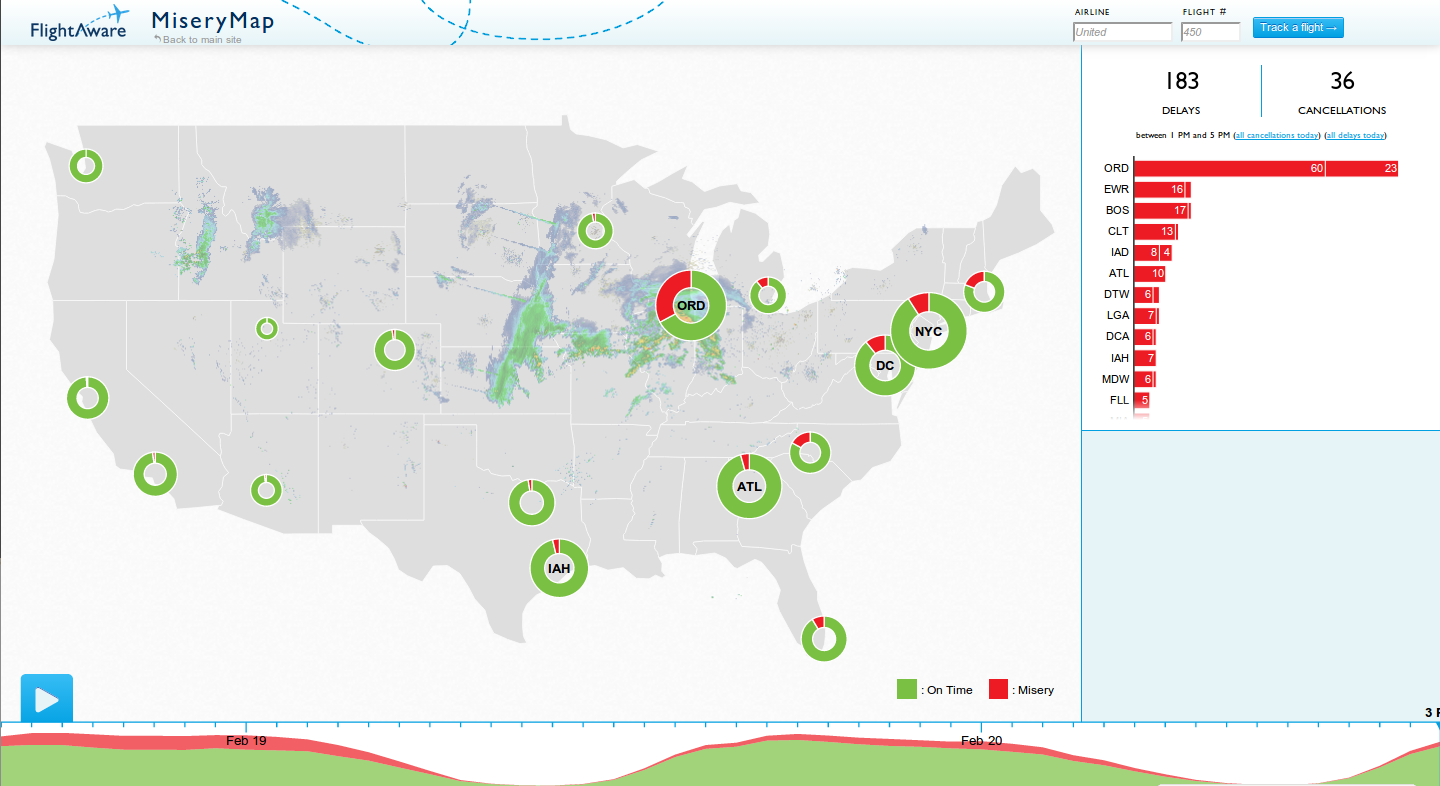
\includegraphics[width=\textwidth,center]{MiseryMap.png}
	\caption[MiseryMap]{MiseryMap \cite{flightAware:MiseryMap}}
	\label{fig:miserymap}
\end{figure}
 
